\chapter{Theory}
% Hier folgt eine kurze Einleitung in die Thematik der Bachelorarbeit.
% Die Einleitung muss kurz sein, damit die vorgegebene Gesamtlänge der 
% Arbeit von 25 Seiten nicht überschritten wird. 
% Die Beschränkung der Seitenzahl sollte man ernst nehmen,
% da Überschreitung zu Abzügen in der Note führen kann. 
% Um der Längenbeschränkung zu genügen, darf auch nicht an der Schriftgröße,
% dem Zeilenabstand oder dem Satzspiegel (bedruckte Fläche der Seite) manipuliert werden.

\section{A General Overview of the IceCube Detector}
The IceCube neutrino detector is a cubic kilometer scale particle detector located near the Amundsen-Scott South Pole Station. The primary goal of 
the detector is the detection of high energy neutrinos as messenger particles for the study of astrophysical sources. The detector unit is split into three 
parts, which are the In-Ice Array, the IceTop, and the DeepCore. 

The In-Ice Array is the largest component and consists of 86 vertical strings, extending vertically into the ice below the surface for \SI{2450}{\metre}. 
Each of the strings contains 60 Digital Optical Modules (DOMs) starting from a depth of \SI{1450}{\metre} all the way down to \SI{2450}{\metre}
The DOMs are evenly separated by \SI{17}{\metre} alongside their respective string, making a total number of \num{5160} DOMs. 

IceTop, as the name suggests, is located at the surface of the ice with \num{162} tanks filled with ice and equipped with PMTs. 
The tanks are arranged in 81 stations in a manner that approximately mimics the structure of the In-Ice Array. 

DeepCore is a sub-array within the In-Ice Array and is located at depths beneath \SI{1750}{\metre}. It contains an extra \num{8} strings alongside the 
\num{7} strings from the In-Ice Array. This creates a more densly packed arrangement of DOMs in the lower center of the detector, which increases its 
ability to detect low-energy signals.

Figure~\ref{fig:icecube_sketch_01} shows a visual representation of this structure. For more details on the structure and build of the detector, see \cite{einstein}.

\begin{figure}[htbp]
    \centering
    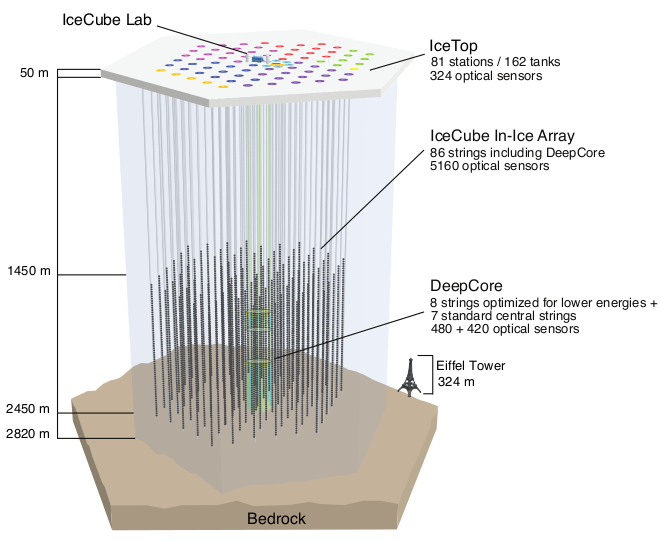
\includegraphics[width=0.7\textwidth]{content/pictures/icecube_sketch_01.png}
    \caption{An overview of the arrangement inside of the detector.}\label{fig:icecube_sketch_01}
\end{figure}

\section{Digital Optical Module}\label{sec:dom}

A single DOM consists of a glass housing, containing the PMT and the corresponding circuit boards. The technical part of the functionality of 
the circuit boards are not of interest for this analysis, so I will not go into detail on that topic. The PMT however is the actual detecting unit of 
the DOM~. A sketch of a PMT is shown in figure~\ref{fig:pmt01}.

\begin{figure}[htbp]
    \centering
    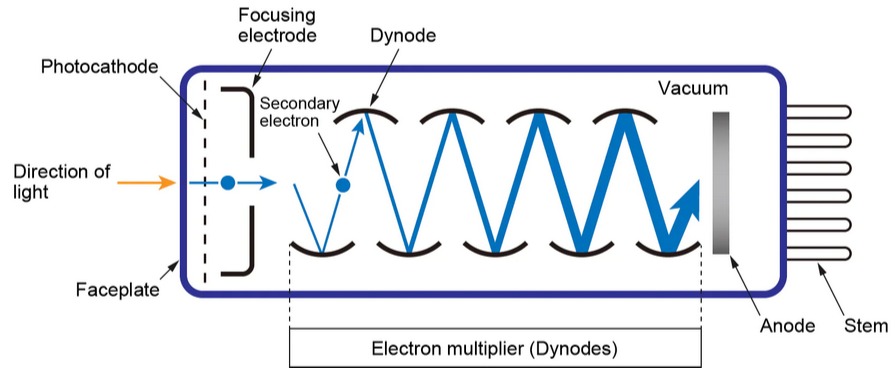
\includegraphics[width=\textwidth]{content/pictures/pmt_sketch_01.png}
    \caption{The principle construction of a photomultiplier.}\label{fig:pmt01}
\end{figure}

When a photon with sufficient energy hits the photocathode of the PMT, its energy is absorbed and an electron is emitted via the photoelectric effect.
The electron is accelerated towards the first dynode due to its electric charge. Hitting the dynode triggers secondary emittions, increasing the total 
number of electrons emitted. This process repeats itself for the number of dynodes the PMT accompasses. After the final amplification by the last 
dynode the electrons are collected by the anode, which produces a current proportional to the intensity of the initial light signal, meaning the amount of
photons hitting the PMT\@. 

\section{Cherenkov Radiation}

The light detected by the photomultipliers is only a secondary signal called Cherenkov radiation~\cite{einstein}. It is created when a charged particle travels through a 
dielectric medium with a velocity greater than the speed of light inside of this medium. The charged particle polarizes the medium's molecules in its
immediate surroundings while passing through it. The excited molecules then return to their ground state by emitting their superfluous energy as light.
Because the light travels slower than the particle exciting the molecules, the light waves do not interfere destructively, but build a conical shock front 
similar in principle to that of an object moving through air at supersonic velocities. This cone of light is the Cherenkov radiation detected by the PMTs.
As explained in section~\ref{sec:dom}, the measured charge is proportional to the intensity of the Cherenkov radiation, which itself is proportional to the 
energy lost by the particle inducing the radiation. Another important value is the angle of the cherenkov light cone, which is dependent on the velocity of the 
particle creating it. This relation is given by 
\begin{equation}
    \cos{\theta_c} = \frac{c}{nv},
\end{equation}
where $n$ is the refractive index of the medium. A higher velocity will therefore lead to a larger angle and vice versa, which, together with the information about 
the charge deposited in the DOMs, enables the possibility of recreating the detected particle's characteristics.

\section{Muons}\label{sec:muons}

A significant percentile of the particles measured in IceCube are muons, which are elementary particles categorized as leptons by the standard model.
This means they carry an electric charge of $\pm 1e$ and have spin $\frac{1}{2}$. The mass of the muon is \num{105.658}\text{MeV}. IceCube detects
muons at a rate of roughly \SI{2500}{Hz}. When cosmic rays collide with the atmosphere's molecules, a multitude of secondary particles are created including 
pions and kaons. The average lifetime of these mesons are of the magnitude of \SI{e-8}{s} or less. Their resulting decay products include muons which are 
produced via the following decay modes:\\

\begin{align}
    \pi^\pm \to \mu^\pm + \nu_\mu \\
    K^\pm \to \mu^\pm + \nu_\mu
\end{align}

These muons have an average lifetime of about \SI{2.2}{\micro\second}, which allows a significant fraction of them to reach the Earths surface due the their 
ultrarelativistic velocities. Details on the effects of relativistic velocities on spacetime can be found in~\cite{einstein}. When a muon travels through the ice 
within the IceCube detector, it produces Cherenkov radiation due to its charge and high velocities and 
can thus be indirectly measured. Realisticly, muons which hit the detector are usually clustered up in bundles, since the cosmic rays responsible for their production
mostly create multiple secondary particles which then decay into muons. Analyzing the cumulative energies of these bundles can provide some insight into the primary 
energies of the original cosmic rays. For a deeper look into the physical characteristics of muons and their creation in the atmosphere, see~\cite{einstein}.


\section{Data Aquisition}\label{sec:daq}

A single DOM measureing a signal is not able to distinguish between different types of events, since its only capability lies in the detection of a current
caused by photons hitting the PMT\@. In order to distinguish between noise and possible signals stemming from Cherenkov radiation, multiple requirements are
put in place to ensure that the full data of a signal is only saved for those signals that might constitute a real event. The data aquisition systems (DAQ)
is the software complex responsible for filtering signals by different characteristics. The first step for any signal is to scan for so called hard local 
coincidences (HLC). This condition is met when there are multiple hits registered in neighbouring DOMs within a certain time frame.
There are \textit{triggers} implemented which search for multiplicities of HLC hits within a certain time frame and with certain spatial requirements.
The specific requirements for different triggers can be seen in table~\ref{tab:trigger_config}.
The simplest one is the simple multiplicity trigger (SMT), which triggers whenever at least $N$ HLC hits occur within a time frame of some 
\si{\micro\second}. This sets a set of intuitive conditions for grouping a cluster of signals into an event that could be a muon or another 
charged particle emitting Cherenkov radiation. 
Another trigger is the fixed rate trigger (FRT) which is of great importance for this thesis. The FRT does not get triggered 
by any multiplicity of events. It is a timed trigger which reads out the entire detector, meaning all functioning DOMs for \SI{10}{ms}
every \SI{300}{s}. Since there are no other conditions set in place for this trigger, it saves everything being measured during the 
readout time frame. This trigger holds a special significance for the analysis of coincident events in IceCube. 
Analyzing the signals collected by the FRT opens a window into the unfiltered distribution of signals collected by the detector. 
As the FRT's data does not undergo any data reduction, it includes all backround noise as well as all other low energy events. 
Since the FRT has an unusually large readout window compared to other triggers, a single \textit{event}, accompassing all signals measured within the readout window,  
is split into multiple \textit{subevents}. On a time scale, these subevents are individual segments within the event, in which a significant signal is detected. 
The identification of subevents is an automated process(?). Hypothetically speaking, if the diagnoses of relevant subevents happens flawlessly, filtering out 
the subevents would yield a clear picture of the noise distribution in IceCube. 



\begin{table}[htbp]
    \vspace{0.5cm}
    \centering
    \renewcommand{\arraystretch}{1.3} % Adjust row height for better spacing
    \setlength{\tabcolsep}{6pt} % Adjust column spacing for better alignment
    \resizebox{\textwidth}{!}{
    \begin{tabular}{@{}llclcl@{}}
    \toprule
    \textbf{Trigger} & \textbf{DOM set}    & \textbf{\(N\) HLC hits} & \textbf{Window (\(\mu s\))} & \textbf{Topology} & \textbf{Rate (Hz)} \\ \midrule
    SMT              & in-ice              & 8                       & 5                          & ---               & 2100               \\
    SMT              & DeepCore            & 3                       & 2.5                        & ---               & 250                \\
    SMT              & IceTop              & 6                       & 5                          & ---               & 25                 \\
    Volume           & in-ice              & 4                       & 1                          & cylinder (\(r=175\,\mathrm{m}, h=75\,\mathrm{m}\)) & 3700               \\
    Volume           & IceTop infill       & 4                       & 0.2                        & cylinder (\(r=60\,\mathrm{m}, h=10\,\mathrm{m}\))  & 4                  \\
    String           & in-ice              & 5                       & 1.5                        & 7 adjacent vertical DOMs                    & 2200               \\
    SLOP             & in-ice              & \(N_{\text{triplet}}=5\) & \(\begin{array}{l} T_{\text{prox}}=2.5,\\ T_{\min}=0,\\ T_{\max}=500 \end{array}\) & \(\begin{array}{l} \alpha_{\min}=140^\circ, v_{\text{rel}}^{\max}=0.5\end{array}\) & 12 \\
    FRT              & all                 & ---                     & ---                        & ---               & 0.003              \\ \bottomrule
    \end{tabular}}
    \caption{Trigger configurations and their parameters.}
    \label{tab:trigger_config}
\end{table}

% \begin{figure}[htbp]
%     \centering
%     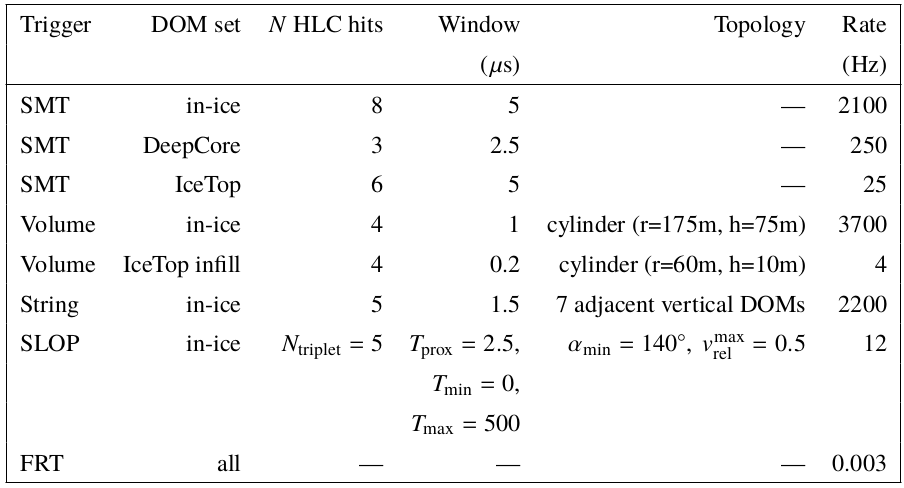
\includegraphics[width=\textwidth]{content/pictures/trigger_list.png}
%     \caption{A list of all triggers in IceCube.}\label{fig:triggers}
% \end{figure}

\section{Coincident Events}\label{sec:coin}

The primary goal of this thesis is the analysis of coincident events in IceCube. This is not to be confused with coincident signals or hits, which are used 
to determine if indeed an event is constituted by the signals. A coincident event however means that two or more muons or muon bundles from different primary 
particles hit the detector within the 
time frame of a readout window from some trigger. The SMT for example will group together any multiplicity of HLC hits in the detector and categorize them as one
event, as long as no other measures are taken. If there are multiple muon bundles resulting from different primary particles, this information would be lost 
and the resulting compound signal would be forwarded as one event. In the case of multiple muons from different sources, this information would be lost. \\
Firstly, an estimation can be made about the percentile of coincident events for any given event rate. As a generic model for the distribution of coincident 
events on a scale of the total event rate, a poisson distribution is a sensible approach. 

\begin{equation}
    P_{\lambda}(k) = \frac{\lambda^k}{k!}\text{e}^{-\lambda} \; .
\end{equation}\\

$\lambda$ is the expected value, which can be rewritten as \\

\begin{equation}
    \lambda = R \cdot \tau \; ,
\end{equation}\\

where $R$ is the rate of incoming particles and $\tau$ is the search time frame set by the trigger, as explained in section\.~\ref{sec:daq}. 
The value of interest is the probability for 2 or more particles hitting the detector within a certain time frame. This yields \\

\begin{equation}
    P_{\lambda = R\cdot\tau}(k\geq2) = e^{- R\cdot\tau} \cdot \sum_{k=2}^\infty \frac{{(R\cdot\tau)}^k}{k!} \; .
\end{equation}\\ 

Multiplying with the event rate $R$ then yields the coincidence rate $R_{co}$ depending on the event rate and the readout window $\tau$:

\begin{equation}
    R_{co}(R,\tau) = R \cdot e^{- R\cdot\tau} \cdot \sum_{k=2}^\infty \frac{{(R\cdot\tau)}^k}{k!}\;.
    \label{eq:multi_rate}
\end{equation}\\

This makes for a useful connection between the coincidence event rate and any spectrum that has a known or easily producible relation to a certain event rate.

% \section{Different spectrums for visualizations}\label{sec:spec}
% % energy spectrum and zenith angle spectrum ? 
% The majority of graphics shown in the analysis part of this thesis, are some variables of interest on either one of the following spectrums. I will thus briefly 
% explain the theory behind their physical meanings in the context of the IceCube detector. 

% \subsection{The Energy Spectrum}
% Energy as a direct observable in IceCube is not something one has access to when analyzing 'real' data, meaning acutal measurements from the detector. 
% This has to do with the way that the events of interest are only indirectly measured. While the energies of certains events can be recreated from the raw data
% collected, another way of accessing energy as a variable is to work with simulated data. 
% For any plot in this thesis, that shows an energy spectrum, simualted monte carlo data is used. 
% For a deeper look into the energy distribution of muons in IceCube, see~\cite{einstein}. 

% \subsection{The Zenith Angle Spectrum}
% Muons created in the atmosphere have differing lengths to travel before they hit the surface, depending on their angle, at which they move towards the surface. 
% In short, this leads to more muons being detected at a zenith angle of \SI{90}{\degree} relative to the surface of the Earth, while with sharper angles, the 
% count rate, as well as their energy, declines. Refer to~\cite{einstein} for more details. 

% \subsection{The Charge Spectrum}
% For the analysis of the events in the FRT, the energy of an event is directly accessible. Therefore, the charge deposited in the detector is used as the 
% spectrum on which to show various measures of interest. As briefly mentioned in section~\ref{sec:muons}, the charge value of a signal is a significant 
% measurement for the recreation of the energy, which is why it is a reasonable measure to use as a spectrum for counting events. 
